\section{Aufbau der Anwendung}

Aus den im vorigen Abschnitt genannten Funktionen lassen sich die folgenden Anforderungen an die Anwendung ableiten: Es muss möglich sein, Veranstaltungen anzulegen und zu diesen Veranstaltungen wiederum Fragen, die von Teilnehmern dieser Veranstaltung beantwortet werden können. Das Antworten soll dabei während der Veranstaltung möglich sein, die Auswertung der Ergebnisse während und nach der Veranstaltung. Die Fragen müssen in eine zeitliche Reihenfolge gebracht werden können. Zur Bewertung der Präsentation sollten deren Folien in der Anwendung verfügbar sein. Zusätzlich ist es wünschenswert auch freie Kommentar zu Veranstaltungen zu erhalten, die Teilnehmer können so z.B. auf Fehler in einer Präsentation hinweisen oder unklare Aspekte aufzeigen.

\subsection{Datenmodell}

\begin{figure}[htb]
\begin{center}
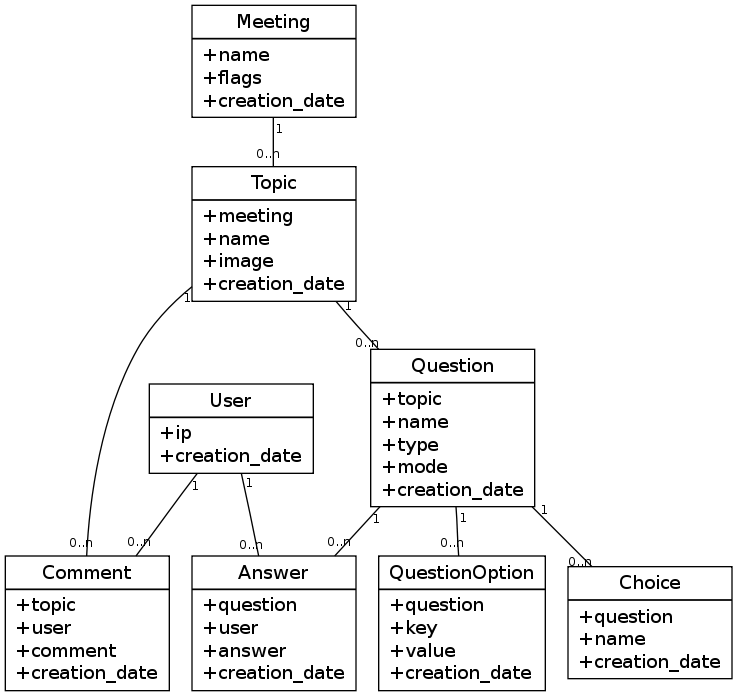
\includegraphics[width=0.75\textwidth]{media/models.png}
\end{center}
\caption{Datenmodell der Anwendung}
\label{f:models}
\end{figure}

\emph{GroupMood} wurde so entwickelt, dass, in eine gewissen Rahmen, beliebige Anwendungsfälle abgebildet werden können. Abbildung~\ref{f:models} zeigt das zugrundeliegende Datenmodell. Die Basis bildet hierbei immer ein \emph{Meeting}, also ein Zusammentreffen von mehreren Personen. Im Verlauf dieses Meetings können verschiedene Arten von Fragen (\emph{Question}) gestellt werden, wobei eigentlich nur zwei Arten von Fragen auftreten. Bei \emph{Von-Bis-Fragen} wählt der Teilnehmer die Antwort auf einem vorgegebenen Zahlenbereich aus. Es kann sich dabei um eine Jahreszahl handeln, z.B. "`Wann ist Napoleon gestorben? Wählen Sie zwischen 1800 und 1900"' oder auch um die Frage nach einer Bewertung "`Wie gut hat ihnen diese Veranstaltung gefallen? Wählen Sie auf einer Skala von 1 bis 10"'. Bei \emph{Auswahl-Fragen} ist der Freiheitsgrad soweit eingeschränkt, dass die Antwort aus einer Auswahl von Antwortmöglichkeiten (\emph{Choice}) ausgewählt werden muss, z.B. "`Wie heißt der aktuelle Bundespräsident? Johannes Rau, Horst Köhler oder Christian Wulff"'. Bei diesem Typ ist es üblich auch mehrere Antwortmöglichkeiten zu zu lassen, z.B. "`Albert Einstein war: Deutscher, vom Sternzeichen Löwe, Physiker. Wählen Sie alle korrekten Antworten"'.

Wie oft eine Antwort pro Teilnehmer dabei abgegeben werden kann, lässt sich ebenfalls mit nur zwei Fällen umfassend beschreiben. So können Antworten entweder einmal pro Frage und Teilnehmern abgegeben werden, oder ständig. Letzteres macht nur bei \emph{Von-Bis-Fragen} Sinn, da hier die abgegebenen Antworten gemittelt werden. Diese Art von Frage ermöglicht die laufende Bewertung eines Meetings, bei denen die Teilnehmer während des Meetings ihre Bewertung jederzeit anpassen können. Tabelle~\ref{table:questiontypes} liefert eine Übersicht über die möglichen Fragetypen und die jeweiligen Einstellungen mit denen diese konfiguriert werden.

Um Fragen im Verlauf einer Veranstaltung passend anzeigen zu können, müssen diese in eine Reihenfolge gebracht werden können. Die Reihenfolge der Fragen wird dabei mit Hilfe von Themen (\emph{Topic}) gruppiert. Ein Thema kann dabei das gesamte Meeting, aber auch eine einzelne Präsentationsfolie sein. So ist es möglich den Ablauf der einzelnen Fragen flexibel fest zu legen und an den jeweiligen Anwendungsfall an zu passen. Zusätzlich ist es möglich, einem Thema ein Bild zu zuweisen, so dass hierüber die Bewertung von Folien einer Präsentation möglich ist.

Neben der Fragen gibt es mit Freitext-Kommentare (\emph{Comment}) eine weitere Möglichkeit, Feedback zu hinterlassen. Kommentare werden dabei wie die Fragen immer zu Themen abgegeben.

Mithilfe von \emph{Flags}, die auf dem Meeting gesetzt werden können, ist es Möglich das Verhalten der App anzupassen, die dann bestimmte Zusatzfunktionen anzeigen kann. Beispielsweise gibt es für die Teilnehmer einer Foto-Abstimmung die Möglichkeit, selber Themen mit Bildern anzulegen.

\begin{table}
\begin{center}
\begin{tabular}{l l l c c c c}
& & & \multicolumn{4}{c}{QuestionOption} \\
& \multicolumn{2}{c}{Question} & \multicolumn{2}{c}{Anzahl Optionen} & \multicolumn{2}{c}{Wertebereich} \\
Frage-Typ & type & mode & min & max & min & max \\
\hline
Single-Choice & choice & single & 1 & 1 & --- & --- \\
Multiple-Choice & choice & single & $\geq$1 & $\geq$min & --- & --- \\
Wert-Auswahl & range & single & --- & --- & $\geq$0 & >min \\
Bewertung & range & average & --- & --- & $\geq$0 & >min \\
\end{tabular}
\caption{Mögliche Fragen und deren Konfiguration}
\label{table:questiontypes}
\end{center}
\end{table}

\subsection{Umsetzung}

\begin{figure}[htb]
\begin{center}
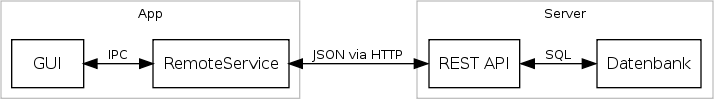
\includegraphics[width=\textwidth]{media/system.png}
\end{center}
\caption{Aufbau des Systems}
\label{f:system}
\end{figure}

Mit \emph{GroupMood} sollen vielen Teilnehmer gleichzeitig an Umfragen teilnehmen können. Um die theoretisch sehr große Anzahl gleichzeitiger Anfragen performant verarbeiten zu können, findet die Kommunikation zwischen den einzelnen Teilnehmern über einen Server statt. Dort werden auch die erzeugten Daten in einer Datenbank gespeichert. Die App greift auf diese Daten über eine \emph{RESTful} HTTP-Schnittstelle zu. Um eine saubere Trennung zwischen GUI-Code und dem Zugriff auf den Server zu erreichen findet jegliche Kommunikation in einem \emph{RemoteService} statt, der von den einzelnen \emph{Activities} der App gebunden wird. In Abbildung~\ref{f:system}  ist der Aufbau des Systems schematisch dargestellt. Die App ist dabei nicht an die Verwendung eines bestimmten Servers gebunden -- sie akzeptiert URLs mit dem Protokoll \texttt{grpmd}, bzw. \texttt{grpmd+ssl} und verwendet diese, um daraus die HTTP(S)-URL zum Server zu generieren (siehe Tabelle~\ref{table:urlschema}).

\begin{table}[htb]
\begin{center}
\begin{tabular}{l l}
\emph{GroupMood}-URL & Server-URL \\
\hline
\texttt{grpmd://<host>/<id>} & \texttt{http://<host>/groupmood/meeting/<id>} \\
\texttt{grpmd+ssl://<host>/<id>} & \texttt{https://<host>/groupmood/meeting/<id>} \\
\end{tabular}
\caption{Umwandlung \emph{GroupMood}-URL in Server-URL}
\label{table:urlschema}
\end{center}
\end{table}

Um die Serialisierung und Deserialisierung zu vereinfachen verwendet das Datenformat JSON-LD\footnote{http://json-ld.org/} hierbei werden die JSON-Daten mit Informationen zum Kontext angereichert, so dass der Verwender erkennen kann, wie die Daten zu interpretieren sind. In der App werden diese Informationen verwendet, um aus den JSON-Daten automatisch die passenden Models erzeugen zu können.

\subsection{Verwendung}

Um an die Daten eines Meetings zu gelangen benötigt die Anwendung eine URL, unter der sie die Daten laden kann. Diese kann z.B. über einen QR-Code übermittelt werden, es ist aber auch möglich, URLs direkt aus Benachrichtigungen oder aus dem Browser zu öffnen. Sind die Daten des Meetings geladen, kann der Benutzer zwischen den einzelnen Themen navigieren. Hierbei sieht er den Namen des Themas oder, falls vorhanden, eine kleine Vorschau der hinterlegten Folie. Die Bilder werden dabei durch den Service im Hintergrund nachgeladen, so kann der Nutzer schnell alle anderen Funktionen der Anwendung verwenden. Die Folienansicht kann auf Vollbildansicht umgeschaltet werden, in der das Bild in höherer Auflösung angezeigt wird, so dass man alle Details der Folie erkennen kann. Zu jedem Thema werden die hinterlegten Fragen angezeigt, durch die mittels einer Wischgeste schnell durchgeblättert werden kann. Je nach Frage-Typ wird ein Werte-Slider oder eine Options-Auswahl angezeigt. Über drei Icons im oberen Bereich des Anwendungsfensters kann zwischen der Darstellung der Fragen, den Kommentaren zu den Fragen und den kumulierten Antworten der Gruppe hin und hergeschaltet werden.

\subsection{GUI-Konzept}

\begin{figure}[htb]
\begin{center}
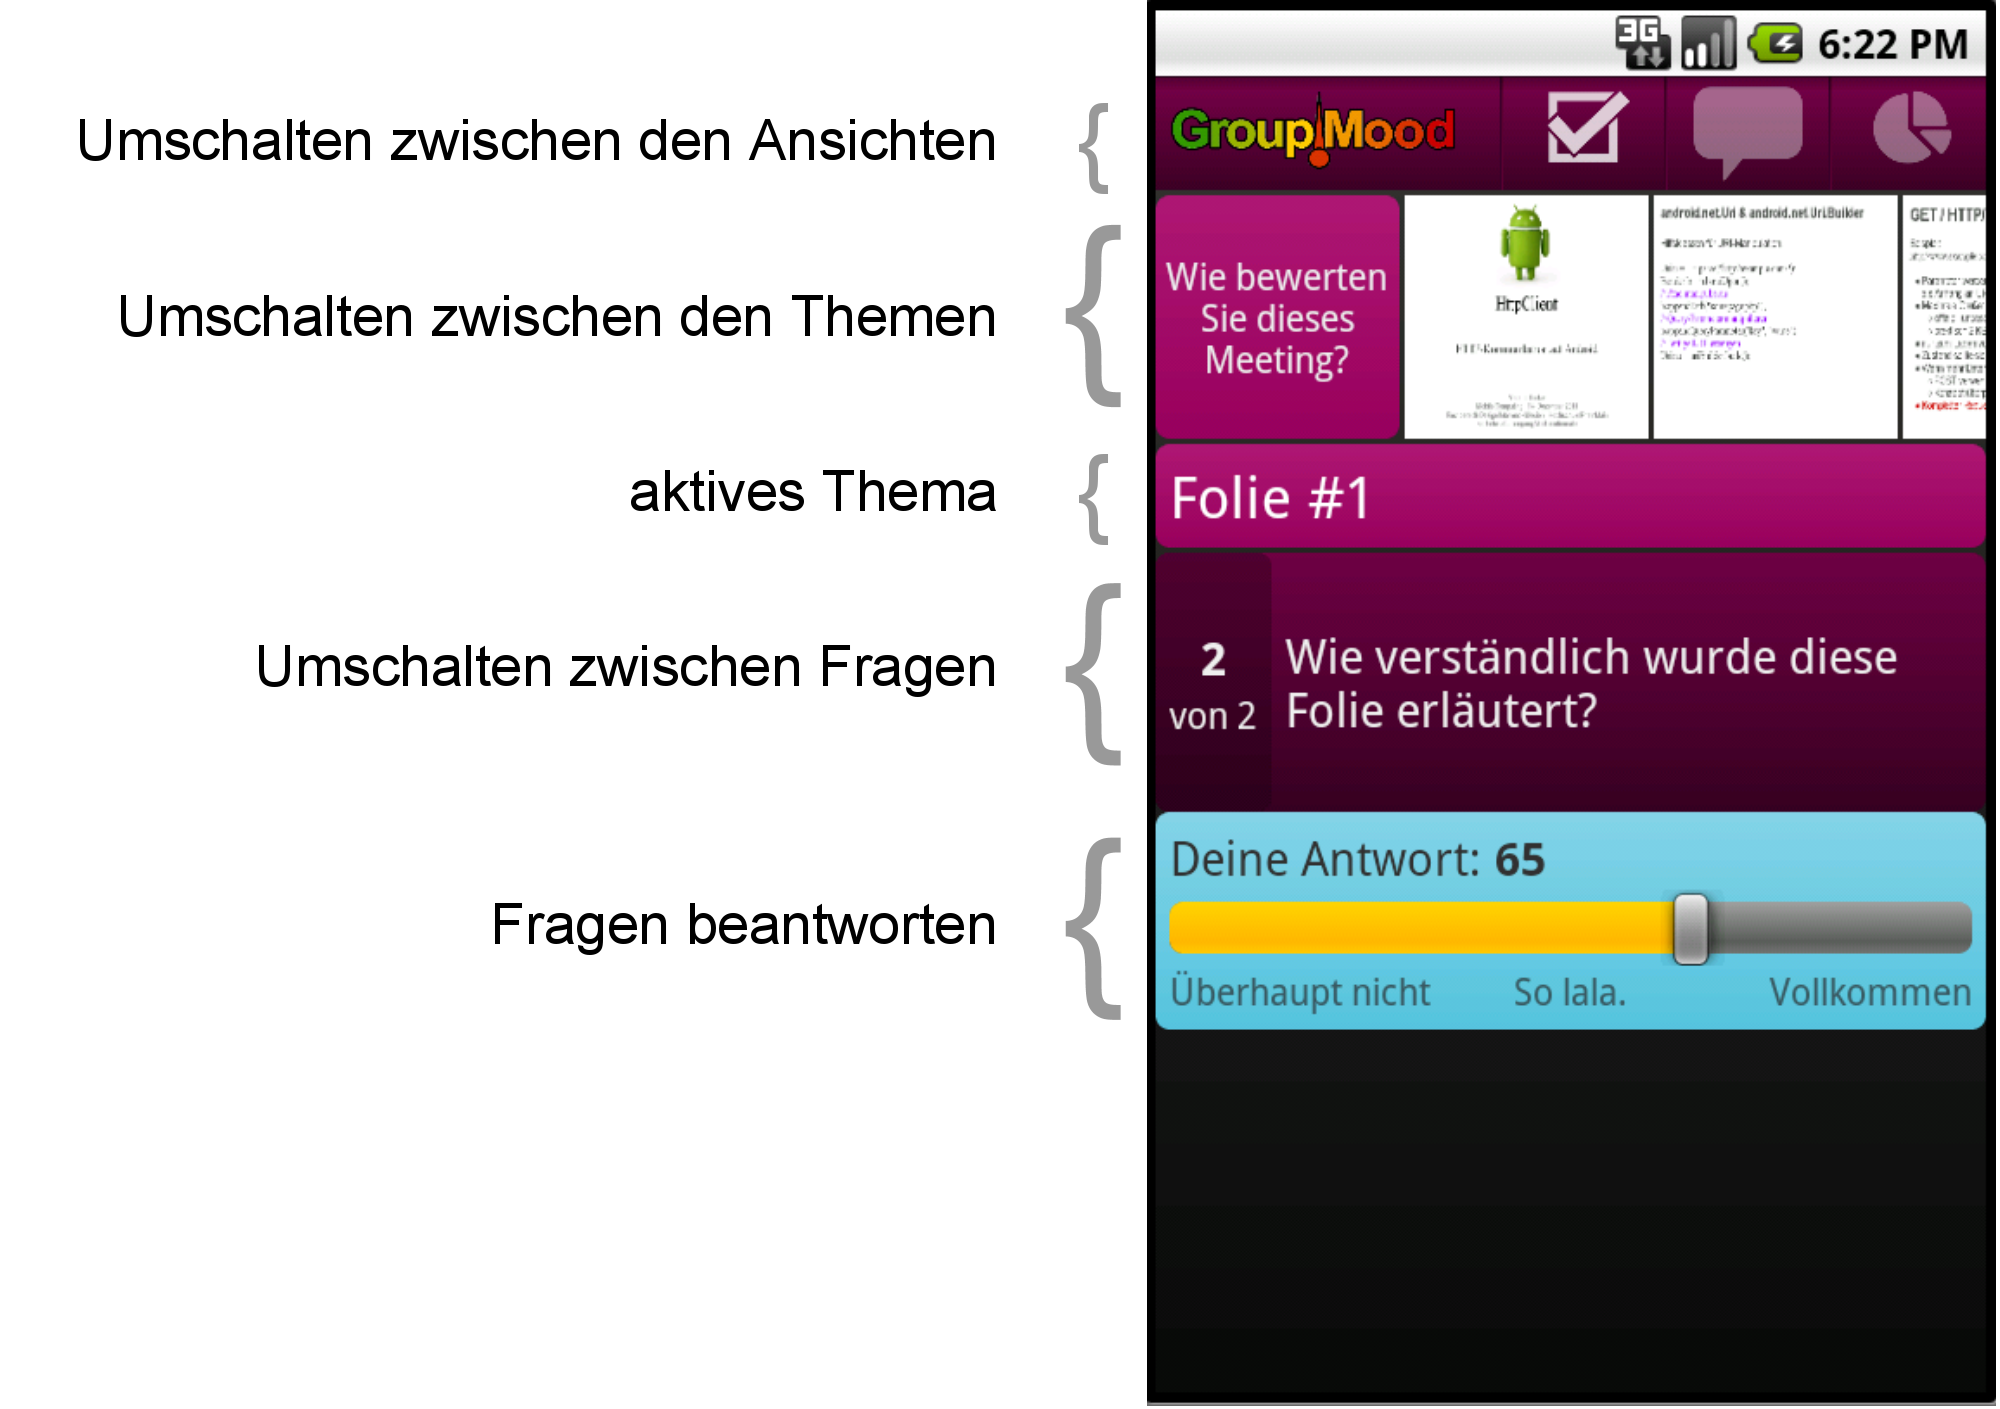
\includegraphics[width=\textwidth]{media/app.png}
\end{center}
\caption{GUI der App}
\label{f:gui}
\end{figure}

Abbildung~\ref{f:gui} zeigt die App in der Darstellung, in der Fragen beantwortet werden. Bei der Gestaltung der App wurde versucht, eine möglichst einfache Bedienung zu ermöglichen -- der Teilnehmer soll nicht von der Veranstaltung abgelenkt werden und schnell die gewünschte Aktion ausführen können. Um dieses Ziel zu erreichen, wurde weitestgehend auf eigene Bedienelemente verzichtet und nur die nativen GUI-Elemente verwendet. Das Navigieren zwischen den einzelnen Themen und deren Fragen erfolgt mit Hilfe einfacher horizontaler und vertikaler Wischgesten, die dem Nutzer allgemein als "`scrollen"' bekannt sind. Um die einfache Orientierung zu unterstützen werden die einzelnen Bereiche der Anwendung farblich unterschieden: informelle Bereiche sind in einem sanften lila gehalten, während die Bereiche, in denen der vom Benutzer Eingaben erwartet werden in einem kräftigen Cyan dargestellt werden.